\documentclass[preprint,5p,times,twocolumn]{elsarticle}
\usepackage{algorithmic,amssymb,graphicx,amssymb,amsmath,psfig,epsfig,subfigure,multirow,url,arcs,proof}
\usepackage[nodots]{numcompress}
\usepackage[linesnumbered,ruled]{algorithm2e}
\usepackage{lineno}
\newtheorem{defn}{DEFENITION}
\newtheorem{theorem}{THEOREM}[section]
\newtheorem{lemma}[theorem]{LEMMA}
\newtheorem{proposition}[theorem]{PROPOSITION}
\newtheorem{obs}[theorem]{OBSERVATION}
\newtheorem{corollary}[theorem]{COROLLARY}
\newtheorem{conjecture}[theorem]{CONJECTURE}

\newenvironment{example}[1][Example]{\begin{trivlist}
\item[\hskip \labelsep {\bfseries #1}]}{\end{trivlist}}
\newenvironment{remark}[1][Remark]{\begin{trivlist}
\item[\hskip \labelsep {\bfseries #1}]}{\end{trivlist}}

\setlength\linenumbersep{3pt}

\journal{Computer \& Graphics}

\begin{document}

\begin{frontmatter}

%% Title, authors and addresses

%% use the tnoteref command within \title for footnotes;
%% use the tnotetext command for the associated footnote;
%% use the fnref command within \author or \address for footnotes;
%% use the fntext command for the associated footnote;
%% use the corref command within \author for corresponding author footnotes;
%% use the cortext command for the associated footnote;
%% use the ead command for the email address,
%% and the form \ead[url] for the home page:
%%
%% \title{Title\tnoteref{label1}}
%% \tnotetext[label1]{}
%% \author{Name\corref{cor1}\fnref{label2}}
%% \ead{email address}
%% \ead[url]{home page}
%% \fntext[label2]{}
%% \cortext[cor1]{}
%% \address{Address\fnref{label3}}
%% \fntext[label3]{}

\title{Title of your report}

%% use optional labels to link authors explicitly to addresses:
%% \author[label1,label2]{<author name>}
%% \address[label1]{<address>}
%% \address[label2]{<address>}

\author{}

\address{}


\begin{abstract}
Write abstarct of your report over here
\end{abstract}

\begin{keyword}
%% keywords here, in the form: keyword \sep keyword
%% MSC codes here, in the form: \MSC code \sep code
%% or \MSC[2008] code \sep code (2000 is the default)

\end{keyword}

\end{frontmatter}

%%
%% Start line numbering here if you want
%%
\linenumbers

\section{Introduction}
 Write the introduction of your report in this section.
 
Figures can also be inserted.  
 
       
  \begin{figure}[!h]
  \centering
  \subfigure[\label{fig:boundarySample}]{
  
\includegraphics[height=1.8in,width=1.2in]{./Images/newSeaHorse1}
                                }
    \subfigure[\label{fig:DotPattern}]{
  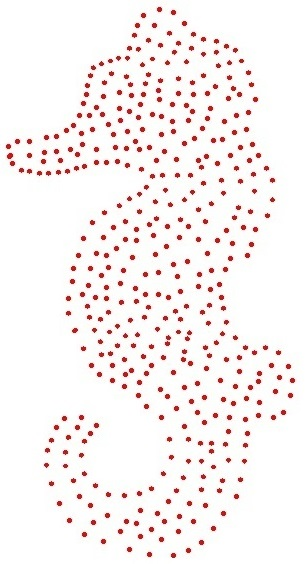
\includegraphics[height=1.8in,width=1.2in]{./Images/NewObjTeaser1}
                              }
  \subfigure[\label{fig:outputCurveReconstruction}]{
 
\includegraphics[height=1.8in,width=1.2in]{./Images/newSeaHorse7}
                              }
  \subfigure[\label{fig:OutputDotPattern}]{
  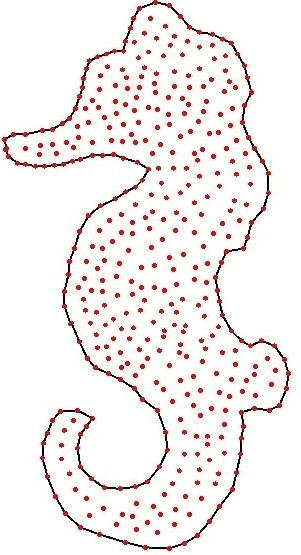
\includegraphics[height=1.8in,width=1.2in]{./Images/NewObjTeaser7}
                                                     }
  \caption{\label{teaser_fig}(a) Boundary sample. (b) Dot pattern. (c,d) Reconstructed shapes of the boundary sample and the dot pattern.}
 
\end{figure}
           
                
           
% % % % % % % % % % % % % % % % % % % % % % % % % % % % % % % % % % % % % % %           
\subsection{}
    If any subsections, write here. References to be saved in references.bib and accessed by cite command. For example CGAL can be referred using  \cite{cgal}. 
    \\
    Entries in bib file can be made by as different categories like article, phd thesis,book,misc etc. as listed in references.bib.

  \subsection{}   
  Any more subsections.
   

           \section{Conclusions and Future Work}
           Write the conclusions of the report
          
           
        

\bibliographystyle{elsarticle-num}
\bibliography{references}

%% Authors are advised to submit their bibtex database files. They are
%% requested to list a bibtex style file in the manuscript if they do
%% not want to use model3-num-names.bst.

%% References without bibTeX database:

% \begin{thebibliography}{00}

%% \bibitem must have the following form:
%%   \bibitem{key}...
%%

% \bibitem{}

% \end{thebibliography}


\end{document}

%%
%% End of file `elsarticle-template-3-num.tex'.
